\subsection{Backend}
\subsubsection{Design pattern utilizzati}
\begin{figure}[H]
\centering
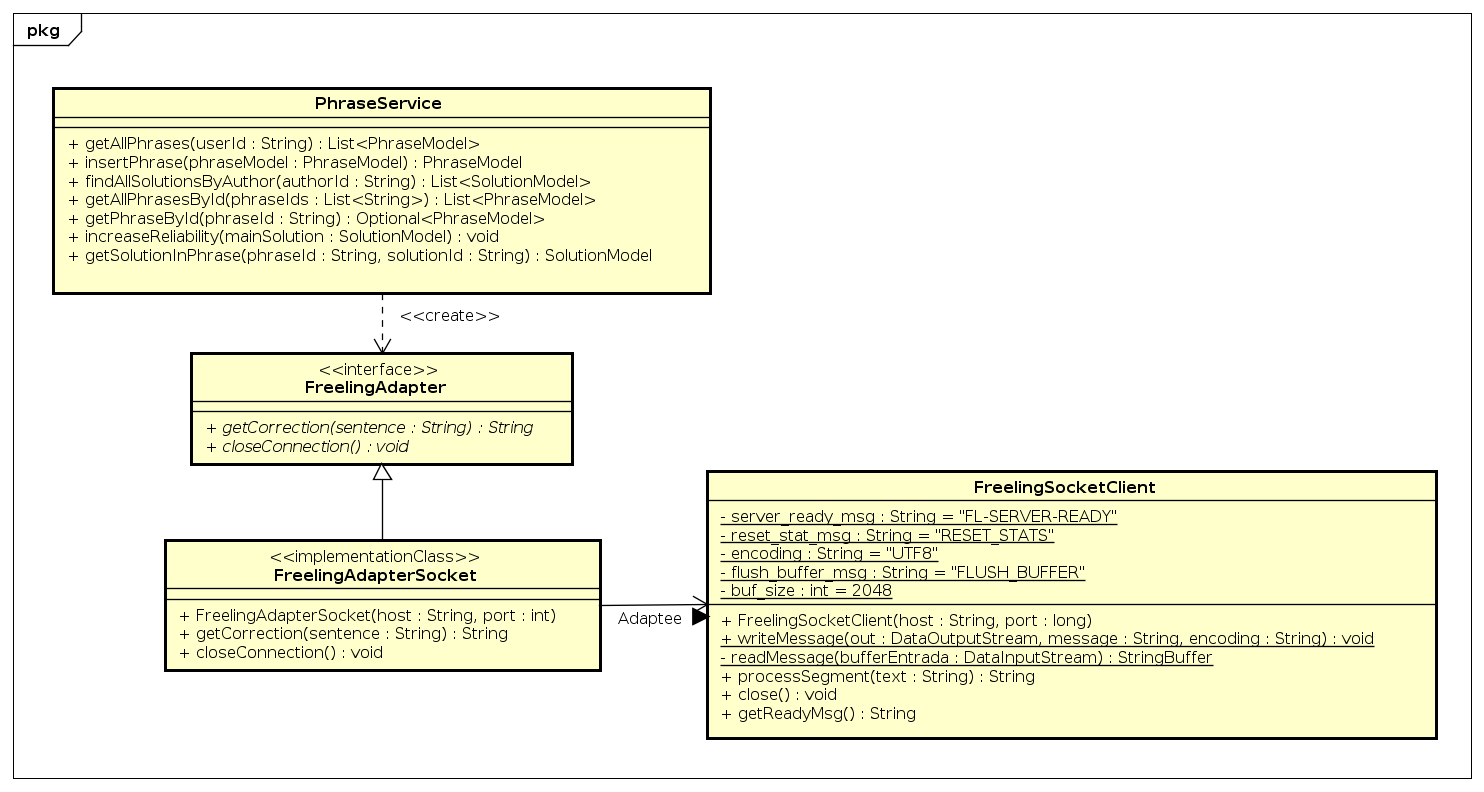
\includegraphics[width=17cm, keepaspectratio]{img/Adapter.png} 
\caption{Object Adapter}
\end{figure}

\subsubsection{MongoDB Database}
\begin{figure}[H]
\centering
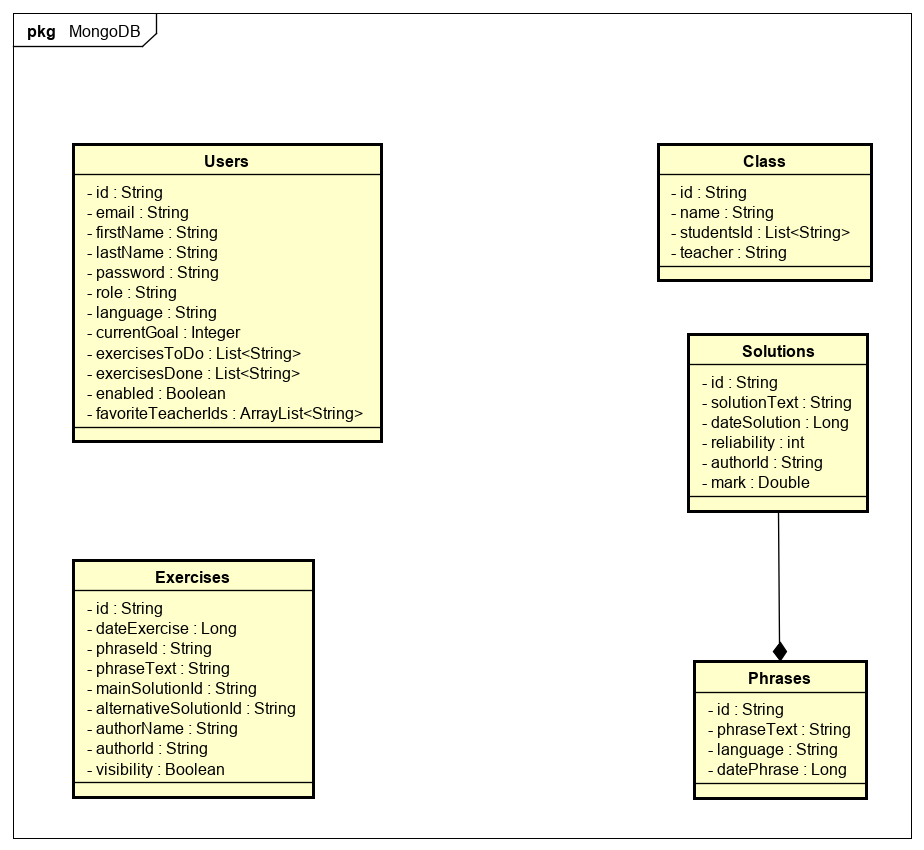
\includegraphics[width=17cm, keepaspectratio]{img/mongodb.png} 
\caption{Exercise insert}
\end{figure}

\subsection{Frontend}
\subsubsection{Design pattern utilizzati}
\paragraph{Flux}\mbox{}\\

\begin{figure}[H]
    \centering
	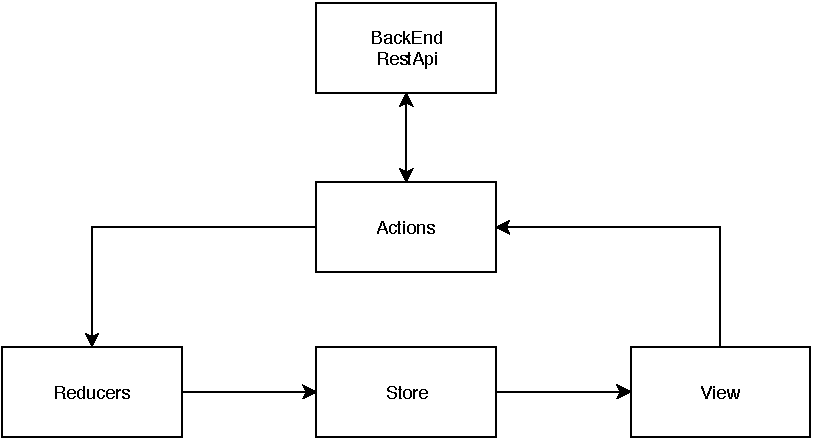
\includegraphics[width=0.7\linewidth]{img/Flux.pdf}
	\caption{Schema del design pattern Flux}
\end{figure}

Per la frontend viene utilizzato React con design pattern Redux, un'evoluzione del design pattern Flux.
In Redux, tutti i dati scorrono in modo unidirezionale attraverso i seguenti componenti:
\begin{itemize}
    \item \textbf{Store: }oggetto immutabile che contiene l'intero stato dell'applicazione in maniera centralizzata;
    \item \textbf{Reducers: }sono funzioni pure. Ogni volta che i Reducer ricevono una nuova azione, 
    processano l'azione ricevuta e, in caso sia necessario apportare delle modifiche allo stato, restituiscono un nuovo oggetto 
    \item \textbf{Action creators: }funzioni che facilitano la gestione del dispatch (creazione di azioni da mandare ai reducers); 
    \item \textbf{View: }componenti grafiche, il loro contenuto dipende dallo store. Sono implementate attraverso un \textit{Observer Pattern} sullo store stesso.
    Ad ogni cambiamento di stato prodotto da un reducers vengono renderizzate le componenti collegate ad esso.
\end{itemize} 

